\chapter{Processo Experimental: seus dados e metadados}
\label{cp:engenharia}

A Engenharia de Software Experimental busca medir e avaliar modelos e tecnologias em contextos práticos, objetivando a obtenção de um corpo de conhecimento. Porém, resultados oriundos de um único experimento não podem estabelecer tal corpo de conhecimento, de modo a determinar fatos sobre um dado fenômeno devido às mais diversas variações que podem ser introduzidas no processo experimental, tais como influências culturais~\cite{Basili99, Miller:2005, Shull03}. Perante a isto, se faz necessário que dados sobre estudos independentes sejam armazenados e compartilhados.

O ato de experimentação consiste no centro do processo científico, a qual representa uma atividade na área de pesquisa científica e se utiliza de métodos de investigação experimental para a condução de experimentos~\cite{Travassos02}. 

Segundo \citeauthoronline{Basili99}~(\citeyear{Basili99}), a experimentação ajuda a determinar a eficácia de métodos e de teorias propostas. Somente experimentos verificam as teorias, podem explorar os fatores críticos, e dar luz ao fenômeno novo para que as teorias possam ser formuladas e corrigidas.

A execução de um experimento requer uma sequência de atividades estabelecidas previamente, que por meio das quais seja possível conduzir um processo experimental de forma precisa e sistemática. Desse modo, \citeauthoronline{Wohlin2012}~(\citeyear{Wohlin2012}) propõem as seguinte organização em fases: 
\begin{itemize}
\item \textbf{Definição} –- estabelece quais são os problemas tratados;
\item \textbf{Planejamento} -– determina-se o projeto, instrumentação e os possíveis riscos para validação dos resultados;
\item \textbf{Operação} –- coleta-se os dados do experimento;
\item \textbf{Análise e Interpretação} –- os dados são analisados e avaliados;
\item \textbf{Apresentação e Empacotamento} -– os resultados são apresentados e suas informações são armazenadas para uso futuro.
\end{itemize}

%\textbf{Definição} -- estabelece quais são os problemas tratados; \textbf{Planejamento} -- determina-se o projeto, instrumentação e os possíveis riscos para validação dos resultados; \textbf{Operação} -- coleta-se os dados do experimento; \textbf{Análise e Interpretação} -- os dados são analisados e avaliados; \textbf{Apresentação e Empacotamento} -- os resultados são apresentados e suas informações são armazenadas para uso futuro. 

Na Figura~\ref{ideia} é apresentado um gráfico com o processo de experimentação adaptado de~\citeauthoronline{Wohlin2012}~(\citeyear{Wohlin2012}): nela é possível observar as fazes, assim como tarefas inerentes a cada uma. 

\begin{figure}[!ht]
\centering
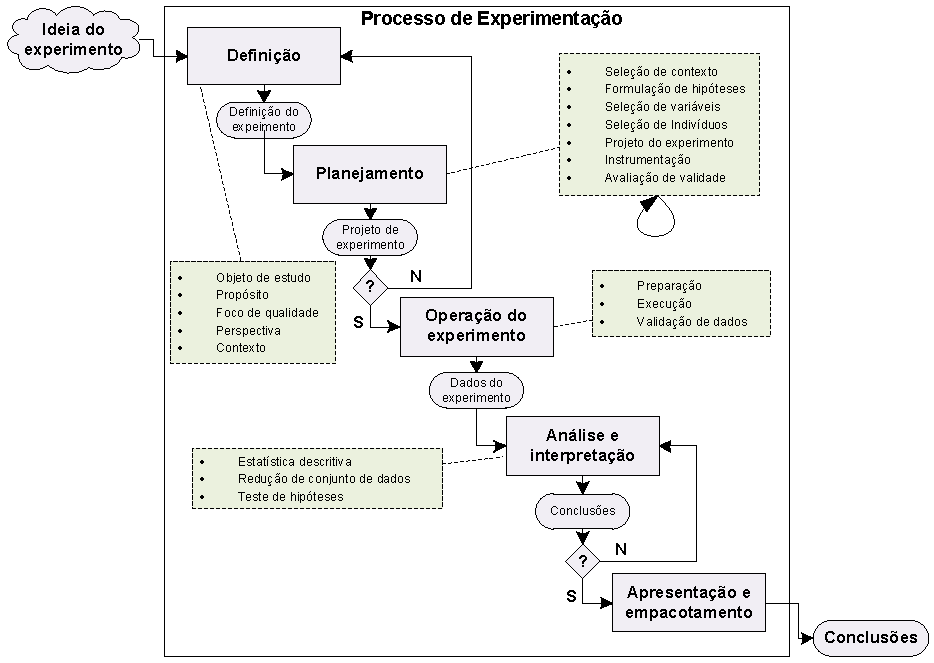
\includegraphics[width=0.98\textwidth]{images/Experimentacao.pdf}
\caption{Processo de Experimentação -- adaptado de~\cite{Wohlin2012}.}
\label{ideia}
\end{figure}

Como apoio, os estudos experimentais atuam como ferramentas para obtenção dos dados necessários através de todo o processo de desenvolvimento de software, almejando resultados objetivos e significativos de forma a alcançar melhorias no processo. Também segundo~\citeauthoronline{Wohlin2012}~(\citeyear{Wohlin2012}), tais estudos podem ser divididos nas seguintes categorias:

\begin{itemize}

\item Pesquisa de opinião: neste primeiro tipo de estudo experimental, busca-se obter dados a respeito de uma técnica ou ferramenta específica, seja uma análise qualitativa ou quantitativa, por meio de entrevistas ou questionários aplicados a uma amostra capaz de representar uma determinada população. Nesta categoria, não controle de execução ou medidas.

\item Estudos de caso: esta categoria é voltada ao monitoramento de atividades, projetos ou tarefas visando observar um atributo específico, ou estabelecer relações entre alguns destes, a qual se prolonga por um determinado período de tempo. Por se tratar uma atividade observacional, o nível de controle é mais elevado do que o anterior.

\item Experimentos controlados: por fim, nesta categoria, o estudo experimental tem sua execução manipulada de forma direta e sistemática, a fim de se ter controle sob todos os elementos que o compõem. Podem ser efetuados experimentos controlados em ambiente universitário, de forma a reduzir custos e riscos do que aplicá-los diretamente à indústria.

\end{itemize}

Somente experimentos verificam as teorias, podem explorar os fatores críticos, e dar luz ao fenômeno novo para que as teorias possam ser formuladas e corrigidas. O processo experimental proporciona de modo sistemático, disciplinado, e controlada a avaliação de processos e de atividades humanas~\cite{Travassos02}.

Através da replicação de experimentos, pesquisadores adquirem conhecimento adicional a respeito dos conceitos estudados. Para que se possa replicar experimentos, é necessário que seu empacotamento seja realizado apropriadamente. Uma replicação em contextos diferentes sujeita o experimento a variações, dentre os quais fatores humanos, socioeconômicos e ambientais do âmbito que o experimento é realizado, possibilitando maior precisão na verificação da validade de hipóteses~\cite{Shull03}. E para a replicação de um experimento, tanto intra quanto extra-grupo~\cite{Mendonca08}, é de suma importância a organização do registro das atividades de um experimento controlado, que são mantidas no chamado \textit{Pacote de Laboratório}.

%%%%%%%%%%%%%%%%%%%%%%%%%%%%%%%%%%%%%%%%
%%%%%%%%%%%%%%%%%%%%%%%%%%%%%%%%%%%%%%%%

\section{Pacotes de Laboratório}
\label{sec:Pacote}
Dentro do âmbito da Engenharia de Software Experimental, a todo momento diversas pesquisas, técnicas e ferramentas são desenvolvidos para validar teses ou otimizar soluções, porém tais recursos ou informações isoladas não formam um corpo de
conhecimento consistente, faz-se necessário compartilhá-los entre os grupos de pesquisa por meio do uso de pacotes de laboratório.

A condução de experimentos controlados ou de suas respectivas replicações, ambas necessitam de validação. A execução destes experimentos, tanto no papel de experimentador quanto de replicador, podem influenciar de forma positiva ou negativa sob muitos aspectos, principalmente em relação ao nível de experiência do condutor do experimento. Por fim, o conjunto de informações obtidos através da execução do processo experimental compõem uma nova instância de pacote de laboratório~\cite{Garcia08}.

Diversos pesquisadores relatam dificuldades na revisão de pacotes de laboratório, como problemas no compartilhamento de conhecimento entre grupos de pesquisa devido uma falta de padronização para a integração de um conhecimento novo e/ou isolado ao conhecimento comum~\cite{Scatalon11}. Desta forma, é imprescindível uma boa definição e construção
de um pacote de laboratório com o uso de uma estrutura específica de simples compreensão, possibilitando inclusive o uso de ontologias para seu desenvolvimento.


%Garcia et al. 
\citeauthoronline{Garcia08} (\citeyear{Garcia08}) propõem o uso de uma ontologia para apoiar a atividade de \textit{Empacotamento} processo de Experimentação no contexto de Engenharia de Software, que descreve os conceitos que compõem um pacote de laboratório para experimentos controlados, chamada \textit{ExperOntology}, apresentada na Figura~\ref{fig:onto01}.
Uma ontologia é uma especificação formal explícita de uma conceitualização compartilhada, definindo parte de um domínio por meio de termos relevantes e seus respectivos relacionamentos, cuja estruturação é baseada por determinadas regras. As regras (axiomas) da \textit{ExperOntology} não são apresentados aqui, mas podem ser observados em~\cite{Garcia08}.
\begin{figure}[!ht]
\centering
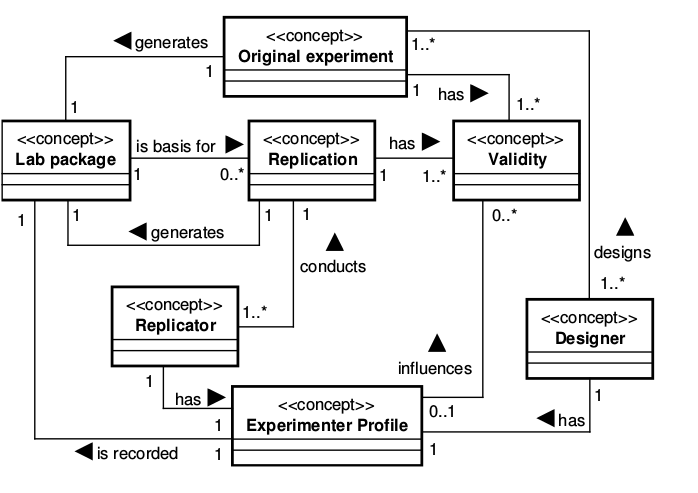
\includegraphics[width=0.8\textwidth]{images/controlados.png}
\caption{Ontologia para Experimentos Controlados~\cite{Garcia08}.}\label{fig:onto01}
\end{figure}

\begin{figure}[!htb]
\centering
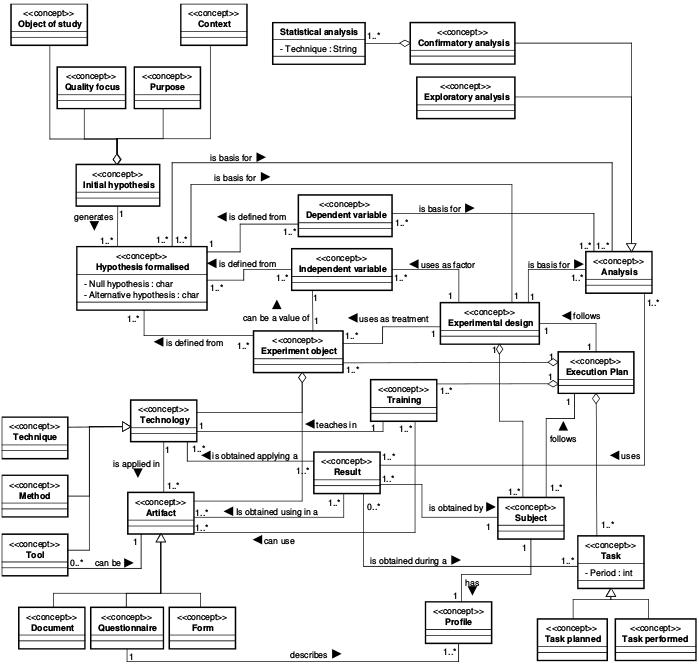
\includegraphics[width=\textwidth]{images/onto.png}
\caption{Ontologia para Pacotes de Laboratório~\cite{Garcia08}.}\label{fig:onto02}
\end{figure}

A \textit{ExperOntology} visa a definir o principais conceitos de experimentos controlados desde a fase de definição até a análise de resultados, sendo importante ressaltar a evolução do experimento e o uso de pacotes de laboratório para armazenamento~\cite{Garcia08}. 

Na Figura \ref{fig:onto02} estão descritos os conceitos que devem fazer parte de um pacote de laboratório, segundo a \textit{ExperOntology}. Inicialmente, é definido um propósito, um contexto, um objeto de estudo e o foco a serem considerados no estudo controlado; en seguida, é elaborada de uma hipótese inicial, a qual juntamente com uma objeto de estudo e um contexto formam a formalização da hipótese. A partir deste ponto, são definidas as hipóteses nulas e alternativas, assim como as variáveis dependentes e independentes. Durante a fase de planejamento, são determinados os objetos de experimentação como as tecnologias e artefatos sob investigação.

O principal objetivo das fases de definição e planejamento é estabelecer um modelo experimental que satisfaça todos os requisitos para a fase de análise. O resultado destas fases culmina em um modelo experimental e no plano de execução, o qual permite a definição de um ambiente controlado, realização de testes das hipóteses e minimização de ameaças para a validação do experimento.

Todos os conceitos apresentados devem ser mantidos no Pacote de Laboratório e, portanto, devem ser instanciados em uma base de dados ou outro meio equivalente para persistir os dados.

\section{Bancos de Dados Não-Relacionais}

Diversas tecnologias para armazenamento de dados têm sido propostas para a persistência de dados, como os Sistemas Gerenciadores de Banco de Dados (\textit{SGBDs}).

O modelo relacional de dados tem sido utilizado em larga escala desde a sua criação. Este modelo tem como característica a utilização de tabelas e tuplas para o armazenamento de dados, assim como o uso de chaves primárias para garantia de unicidade (identificação única de elementos de dados)~\cite{brito2010bancos}.

Mediante ao crescente número de aplicações, o volume de dados tem aumentado exponencialmente nos últimos anos, e com tal crescimento limitações do modelo relacional tem ficado evidente, principalmente quanto à eficiência na recuperação de dados e escalabilidade~\cite{toth2011abordagem}. Para este projeto, a principal limitação é a necessidade de se ter uma estrutura de tabelas pré-definidas, com seus respectivos atributos, o que pode ser uma restrição, pois experimentos controlados podem ter variações nos dados tratados, difícil de ser acomodados em uma estrutura relacional.

Como alternativa, há soluções tecnológicas alternativas que priorizam flexibilidade quanto ao armazenamento, desse modo, não empregam regras presentes no modelo relacional tradicional. Um dessas alternativas é o Modelo Não-Relacional (NoRel), o qual não tem como objetivo substituir o modelo relacional por completo, mas somente em casos em que seja mais vantajoso utilizá-lo, como em ambientes de Big Data. Alguns representantes de base não-relacionais são: Cassandra~\cite{cassandra2014apache}, Dynamo~\cite{sivasubramanian2012amazon}, MongoDB~\cite{banker2011mongodb} e BigTable~\cite{chang2008bigtable}.

Devido à inexistência de regras para a organização dos seus dados, diversas categorias de sistemas de banco de dados não-relacionais tem sido desenvolvidas, os principais são detalhados a seguir.


\begin{itemize}
\item Orientados a Colunas (\textit{Column}): é a categoria que mais se aproxima do modelo relacional, porém todas as suas operações são voltadas para as colunas, ao invés das tuplas como no modelo relacional. O seu grande diferencial está na facilidade de inserção de novas colunas, ou seja, atributos com o sistema já em operação, conforme se tornarem necessários, sem apresentar problemas de esquema ou redundância de dados~\cite{vaish2013getting}.

\item Armazenamento em Documentos (\textit{Document}): nesta categoria cada item é armazenado em um novo arquivo, em geral sua organização é feita através de estruturas chamadas coleções as quais são equivalentes as tabelas no modelo relacional, não possuem qualquer esquema, dois objetos de uma mesma coleção podem ter atributos diferentes, o que permite grande flexibilidade, sendo que cada registro é um arquivo. Os principais formatos de arquivos são JSON, XML, BSON e YAML~\cite{vaish2013getting}.

\item Armazenamento Chave/Valor (\textit{Key/Value}): também muito semelhante à categoria anterior (\textit{Document}), porém seu armazenamento é feito com uso de uma chave, assemelhando-se a uma tabela \textit{Hash}, ou um \textit{array} associativo. Sua grande vantagem é busca por chaves~\cite{vaish2013getting}.

\item Armazenamento em Grafos (\textit{Graph}): esta categoria tem foco nos relacionamentos entre as entidades, que no caso são os nós do grafo, permitindo o uso de múltiplas ligações entre os nós para demonstrar características em comum. Este modelo pode ser ideal para redes sociais. Uma prática usual é a mescla entre o banco de dados orientado a documentos e o orientado a grafos, tornando não obrigatória a presença de relacionamentos~\cite{vaish2013getting}.

\end{itemize}

\begin{table}[!htb]
\centering
\caption{Banco de Dados Não-Relacional e sua tecnologia de armazenamento.}\label{tab:01}
\begin{tabular}{c|c|c|c|c}
\hline
\textbf{Document} & \textbf{Key-Value} & \textbf{XML} & \textbf{Column} & \textbf{Graph}\\ 
\hline                               
MongoDB & Redis & BaseX & BigTable & Neo4J \\
\hline
CouchDB & Membase & eXist & Haddop/HBase & FlockDB \\
\hline
RavenDB & Voldemort & - & Cassandra & InfiniteGraph \\
\hline
\end{tabular}
\end{table}
\normalsize

Na Tebela~\ref{tab:01} há uma breve lista de tecnologias de banco de dados não-relacionais e a respectiva classificação, segundo as classes de armazenamento apresentadas.
Antes de se estabelecer uma comparação entre os modelos, é importante definir conceitos como que deem compor essa comparação, são eles:



\begin{itemize}
\item Escalonamento: este conceito, no contexto de banco de dados, consiste na capacidade em que uma base de dados tem de destruição tanto horizontal (\textit{scale out}), neste caso a estruturação do sistema é dividida em várias máquinas tanto por parte do banco de dados; quanto vertical (\textit{scale up}), no qual são realizadas melhorias de hardware em relação à processamento e armazenamento~\cite{toth2011abordagem}.

\item Consistência: refere-se à capacidade de manter os dados de forma íntegra, de modo que evite quaisquer problemas no banco de dados possam modificar ou corromper os dados armazenados~\cite{brito2010bancos}.

\item Disponibilidade: este quesito se refere a capacidade de acesso do usuário a referida informação, tanto em quesito de velocidade quanto de solicitação~\cite{brito2010bancos}.
\end{itemize}

\begin{table}[!bth]
\label{comparativo}
\centering
\caption{Análise Comparativa do Modelo Relacional e Não-Relacional~\cite{brito2010bancos}.}
\begin{tabular}{l|p{5.7cm}|p{5.7cm}}
\hline
 & \textbf{Relacional} & \textbf{Não-Relacional} \\ 
\hline                               
\textbf{Escalonamento} & Possível, porém complexo devido à natureza estruturada do modelo, a adição de forma dinâmica e transparente de novos nós no modelo não é realizada de modo natural. & Uma das principais vantagens desse modelo, por não possuir nenhum tipo de esquema predefinido, o modelo possui maior flexibilidade o que favorece a inclusão transparente de outros elementos.\\
\hline
\textbf{Consistência} & Ponto mais forte do modelo relacional. As regras de consistência presentes propiciam uma maior grau de rigor quanto à consistência das informações. & Realizada de modo eventual no modelo: só garante que, se nenhuma atualização for realizada sobre o item de dados, todos os acessos a esse item devolvem o último valor atualizado. \\
\hline
\textbf{Disponibilidade} & Dada a dificuldade de se conseguir trabalhar de forma eficiente com a distribuição dos dados, esse modelo pode não suportar a demanda muito grande de informações do banco. & Outro fator fundamental do sucesso desse modelo. O alto grau de distribuição dos dados propicia que um maior número de solicitações aos dados seja atendida por parte do sistema e que o sistema fique menos tempo não-disponível. \\
\hline
\end{tabular}
\normalsize
\end{table}

Por fim, de modo a esclarecer as reais vantagens e desvantagens do uso de uma base de dados não-relacional, na Tabela~\ref{comparativo} é apresentado um comparativo com o tradicional modelo relacional analisando os quesitos de consistência, escalonamento e disponibilidade~\cite{brito2010bancos}.

Perante esta conceituação, a camada de persistência será elaborada utilizando o banco de dados \textit{MySQL}~\cite{mysql2001mysql} devido à utilização da ferramenta \textit{OntoExpTool}~\cite{Pucci2014}, mantendo assim a compatibilidade para os modelos já criados. Para a persistência da camada de interface será utilizada uma estrutura orientada a documentos, utilizando \textit{eXtensible Markup Language} (XML). Tal decisão foi tomada pois a estrutura orientada a documentos  se mostrou adequada tanto para o armazenamento, quanto para a transferência de protocolos experimentais entre exterimentador e replicador. Adicionalmente, essa organização estrutural permite que os dados de um experimentos sejam mantidos em uma base de dados. e seu protocolo, expresso em BPMN (armazenado em XML) possa ser compartilhado, sem expor os dados. O compartilhamento do protocolo juntamente com os dados do experimento (dados coletados) podem ser compartilhados, desde que desejado pelo experimentador (resposável pela criação do experimento e, consequentemente, do seu Pacote de Laboratório).
